\documentclass{report}

\usepackage[francais]{babel}
\usepackage[utf8x]{inputenc}
\usepackage[T1]{fontenc}
\usepackage[final]{pdfpages}
\usepackage{graphicx}
\usepackage{array}
\usepackage{eurosym}
\usepackage{listings}
%\usepackage{gasetex}
\title{Université de Technologie Belfort-Montbéliard\\
Projet LO41\\
Simulation de carrefours routiers intelligents}
\author{Florian Lacour\\
Michael Ayeng}

\lstdefinestyle{customc}{
  belowcaptionskip=1\baselineskip,
  xleftmargin=\parindent,
  language=C,
  showstringspaces=false,
  basicstyle=\footnotesize\ttfamily,
  keywordstyle=\bfseries\color{green!35!black},
  commentstyle=\itshape\color{purple!30!black},
  identifierstyle=\color{blue},
  stringstyle=\color{orange},
}

\lstset{escapechar=@,style=customc}

\begin{document}



\maketitle

\tableofcontents



\chapter{Introduction}
	\paragraph{}
		Dans le cadre de l'UV LO41, architectures et utilisation des systèmes d'exploitation, nous avons étés amenés à réaliser un projet reprenant différents principes vues en cours. L'objectif de celui-ci était la réalisation d'une simulation de carrefours routiers intelligents.
	\paragraph{}
		Cette simulation doit permettre la circulation de manière fluide de véhicules se déplacent de manière autonome dans un ensemble de 4 échangeurs.
	\paragraph{}
		Dans ce rapport, nous nous intéresserons dans un premier temps au cahier des charges du projet, puis aux entités mises en place afin de réaliser ce projet. Enfin, nous verrons plus en détails le fonctionnement et la communication des différentes entités constituantes de la simulation.
	
\chapter{Cahier des charges}
	\paragraph{}
	Afin de remplir les objectifs de ce projet, il nous était demandé de réaliser un programme informatique permettant la simulation d'un ensemble de 4 carrefours routiers intelligents, gérants un trafic de véhicules autonomes. Ces carrefours routiers devaient être orchestrés par un serveur-contrôleur gérant et optimisant les flux du trafic.
	\paragraph{}
	Le développement de ce programme devait être réalisé en langage C, dans un environnement Linux. La bonne gestion de la mémoire, la prise en compte des signaux et la réutilisation de principes de communications vues en cours étaient des objectifs de ce projet.
	\begin{center}
			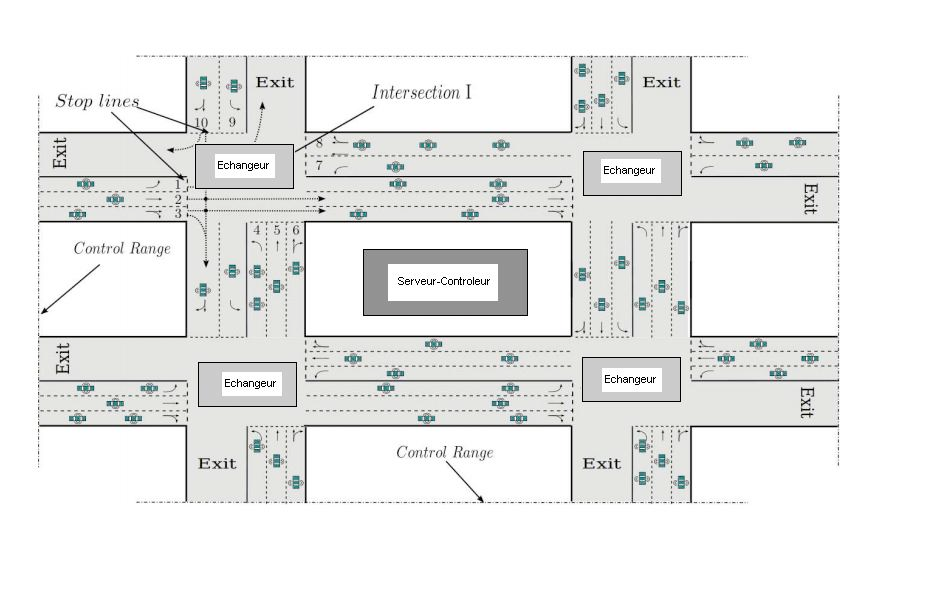
\includegraphics[scale=0.37]{simulation.png}	
			Exemple de structure routière à simuler
	\end{center}
	
	
\chapter{Présentation des entités}

	\section{Les véhicules}
	Dans cette simulation, on suppose les véhicules autonomes sont équipées d'un dispositif embarqué leurs permettant de communiquer avec l'infrastructure routière. Ces véhicules démarrent leur parcours à un échangeur et traversent la simulation jusqu'à sortir par un autre échangeur. A son arrivée aux abords d'un échangeur, le véhicule émet une requête au serveur à l'aide de son dispositif de communication, afin d'être pris en charge.
	
	\section{Les échangeurs}
	Un échangeur ne dispose pas de feux de circulation. A la place, il dispose d'une barrière virtuelle autorisant ou bloquant le parcours d'un véhicule. Ainsi, lorsqu'il en obtient l'ordre du serveur, l'échangeur va ouvrir sa barrière virtuelle et autorisé le véhicule à le traverser. L'échangeur ne peut pas autoriser plusieurs véhicules à le traverser en même temps. Lorsque le véhicule l'informe qu'il à terminer sa traversé, l'échangeur referme la barrière virtuelle.
	
	\section{Le serveur}
	Le serveur dispose d'une vue d'ensemble des échangeurs présent et dispose d'informations concernant leur état. Il connaît également la liste des véhicules qu'il doit gérer. Cette liste représente le trafic de la simulation. En permanence, le serveur est chargé d'être à l'écoute d'un véhicule souhaitant traverser un échangeur. Le serveur recherche un véhicule souhaitant traverser, en utilisant un système de priorité favorisant les véhicules dont le temps d'attente est le plus long. Lorsqu'un véhicule dont l'échangeur est disponible à été trouvé, on autorise l'échangeur à le gérer.
	
	\section{Le générateur de véhicule}
	Un générateur se charge de créer des véhicules dans la simulation. Ce générateur va paramétrer avec des valeurs aléatoires le point d'apparition et le point d'arrivée du véhicule, avec de l'ajouter à la liste de traitement du serveur.

\chapter{Fonctionnement et communication}
	
	\section{Fonctionnement}
	\paragraph{}
	La solution qui à été retenu pour la création de ce programme est l'utilisation d'un unique processus, et d'une multiplicité de threads, chacun représentant une entité de la simulation.
	
	\subsection{Le processus principal}
	\paragraph{}
	Dans le programme réalisé, le processus principal n'a pour fonction que de créer et d’héberger les différents threads et structures du programme. Il sert d'hôte aux entités de la simulation. Il exécute la fonction main contenant les différentes instructions pour mener à bien cette tâche.
	\paragraph{}	
	L'utilisateur transmet au processus via l'argument de lancement du programme le nombre de véhicule qu'il souhaite voir créer dans la simulation. Cette valeur doit être strictement inférieure à 5000. En effet, les test ont montrer que dépasser cette valeur entraîne la création d'erreur dans le programme. Est en cause le nombre maximal de thread que la configuration de l'utilisateur peut gérer.
	Le nombre de véhicule ainsi obtenu est utilisé pour paramétrer la structure du serveur, ainsi que les différents sémaphores servant à la communication (cf. Section "Communication").
	\paragraph{}
	La fonction main du processus est également en charge de paramétrer les structures des échangeurs et d'initialiser les threads du serveur, des échangeurs et du générateur du véhicule.
	Une fois cette tâche accomplie, il attend la fin du thread de génération de véhicule et de chaque thread de véhicule pour correctement nettoyer la mémoire avant la terminaison du programme.
	\subsection{Le thread du serveur}
	\paragraph{}
	Initialisé en mode "détaché" par la fonction main, le thread du serveur à pour but de traiter les véhicules souhaitent se déplacer sur le système d'échangeur, en autorisant les échangeurs correspondant à laisser par les véhicules en question.
	\paragraph{}
	Le thread possède un pointeur sur la structure du serveur, et à donc accès à la liste de véhicule à traité représentant le trafic de la simulation.
	\paragraph{}
	Le thread attend la notification d'un véhicule souhaitant traverser un échangeur pour effectuer une recherche dans sa liste et trouver un véhicule dont l'échangeur est disponible. Si lors de cette recherche, l'échangeur du véhicule trouvé est indisponible, le véhicule verra sa priorité incrémenter, le rendant ainsi plus prioritaire la prochaine fois que le serveur effectuera une recherche.
	\paragraph{}
	Le serveur autorise ensuite le thread de l'échangeur concerné à ouvrir le chemin au véhicule, et rend l'échangeur indisponible.
	\subsection{Les threads des échangeurs}
	\paragraph{}
	Initialisé en mode "détaché" par la fonction main, les threads des échangeurs ont pour but d'ouvrir leur barrière virtuelle et d'autoriser les véhicules le souhaitant à les traverser.
	\paragraph{}
	Les threads possèdes des pointeurs sur leur structure d'échangeur respective. Ils savent donc quel véhicule est en passe de les traverser.
	\paragraph{}
	Les threads attendent l'autorisation du serveur pour ouvrir leur barrière virtuelle, et ensuite autoriser au bon véhicule de les traverser. Ils attendent ensuite la notification du véhicule leur permettant de refermer leur barrière. Ils se rendent ensuite à nouveau disponible.
	\subsection{Le thread générateur de véhicule}
	\paragraph{}
	Initialisé par la fonction main, le thread générateur de véhicule à pour but de générer des véhicules ayant des paramètres aléatoires dans la simulation.
	\paragraph{}
	Le thread dispose du nombre véhicule que l'utilisateur à souhaiter voir générer.
	\paragraph{}
	Après avoir correctement paramétrer la structure du véhicule, le thread généréateur de véhicule va créer un thread pour le véhicule nouvellement créer. Cette tâche va être répéter autant de fois qu'il y a de véhicule à générer. Le thread se terminera ensuite.
	\subsection{Les threads de véhicule}
	\paragraph{}
	Initialisés par le thread générateur de véhicule, les threads de véhicule sont actifs tant que le véhicule qu'ils représentent n'est pas arrivé au bout de son parcours.
	\paragraph{}
	Ils informent le serveur de leur volonté de traverser un échangeur et attende l'autorisation du thread échangeur correspondant. Ils traversent ensuite l'échangeur et le notifie, afin qu'il puisse refermer sa barrière. Il détermine ensuite le prochain échangeur à visiter de manière pseudo-aléatoire (le véhicule tient compte des échangeurs déjà visités, ainsi il ne tournera pas en rond). Si le véhicule est arrivée à la fin de son parcours, le thread se termine.
	\newpage
	\section{Réseau de Pétri}
	Pour plus de clarté nous avont choisi de representer un reseau de petri pour une voiture ainsi que une voiture :
	\begin{center}
	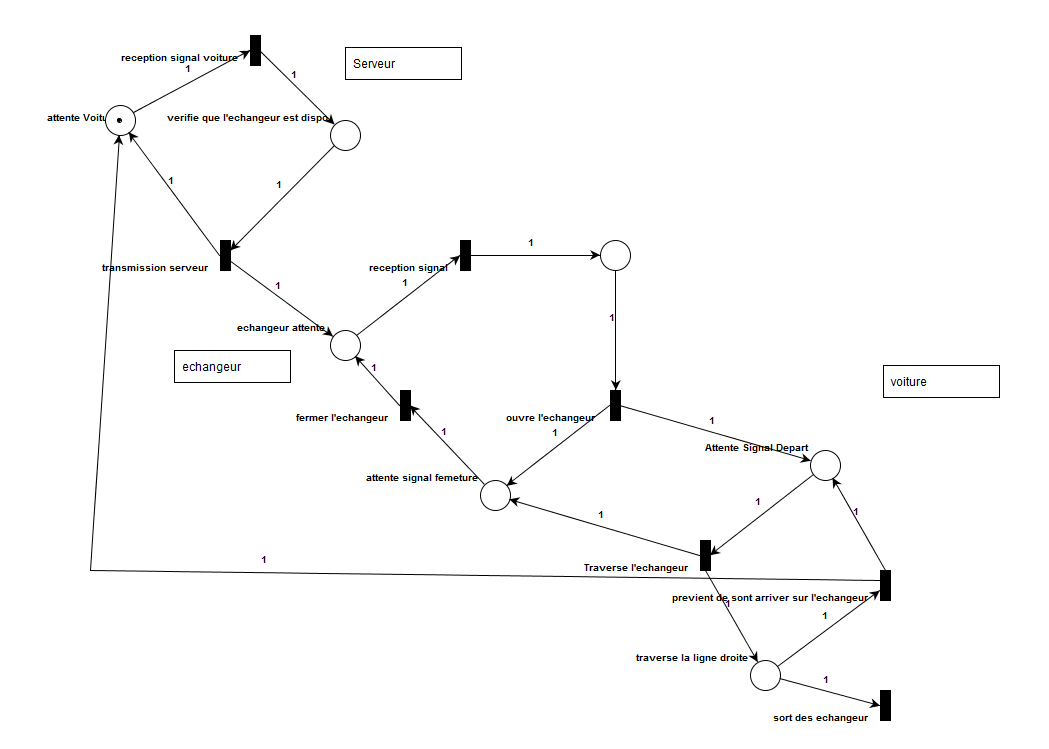
\includegraphics[scale=0.4]{Petri}
	\end{center}
	
		\newpage
	
	\section{Communication}
	\paragraph{}
	Le principe de sémaphore à été employé dans ce programme, afin de permettre la communication entre les différents threads. 
	\paragraph{}
	Une communication employant mutex et signaux à été mis en place pendant le développement du programme, cependant son utilisation était source de dysfonctionnement, car le nombre précis de signaux envoyés par les différentes entités était perdu.
	\paragraph{}
	L'emploi de sémaphore permet de connaître le nombre de fois qu'une notification à été envoyé, et permet ainsi aux threads d'inclure cette valeur dans leurs algorithmes de fonctionnement.
	\paragraph{}
	Tous les sémaphores sont initialisées dès le début du programme, de ce fait il est nécessaire de décider dès le début du programme d'un nombre maximum de voiture a gérer.
	
			\subsection{Les sémaphores des échangeurs}
			Chaque échangeur possède 2 sémaphores, le premier sémaphore permet de connaître le nombre de voiture qui désirent entrer dans le carrefour et de communiquer sur l'ouverture de la barrière, le second sémaphore est utilisé par la voiture pour libérer le carrefour et autoriser l'échangeur à fermer sa barrière.

			\subsection{Les sémaphores des véhicules}
			Les voitures possèdent un sémaphore afin de recevoir le signal de départ de la part de l’échangeur. 

			\subsection{Les sémaphores du serveur}
			\paragraph{}
			Le serveur possède un sémaphore permettant de le prévenir lorsque une voiture demande à traverser un échangeur.
		
		
	

\end{document}
